\documentclass[a4paper]{article}
\usepackage[utf8]{inputenc}
\usepackage[a4paper]{geometry}
\geometry{verbose, marginparwidth=15mm, marginparsep=3mm, tmargin=25mm}
\usepackage{tabulary}
\usepackage{enumitem}
\usepackage{graphicx}
\usepackage{float}

\usepackage{url}
\title{Redbackup: Projectplan}
\author{
		Fabian Hauser \\
		Raphael Zimmermann
}
\date{\today}


\begin{document}
\maketitle

\section{Project Overview}
The goal of the Study Project is to provide a theoretical description of an append-only, distributed peer-to-peer data storage as well as a working prototype as described in the problem statement \cite{problemstatement}.

The project setting, vision, goals, as well as all other project boundaries, are described in depth in the problem statement \cite{problemstatement}.

\section{Project Organization}

The project has a flat structure. All team members have the same strategic rights and duties. Prof. Dr Farhad Mehta is the project supervisor and is therefore superior in the organization chart as visible in Figure \ref{fig:organigram}.

\begin{figure}[H]
	\centering
	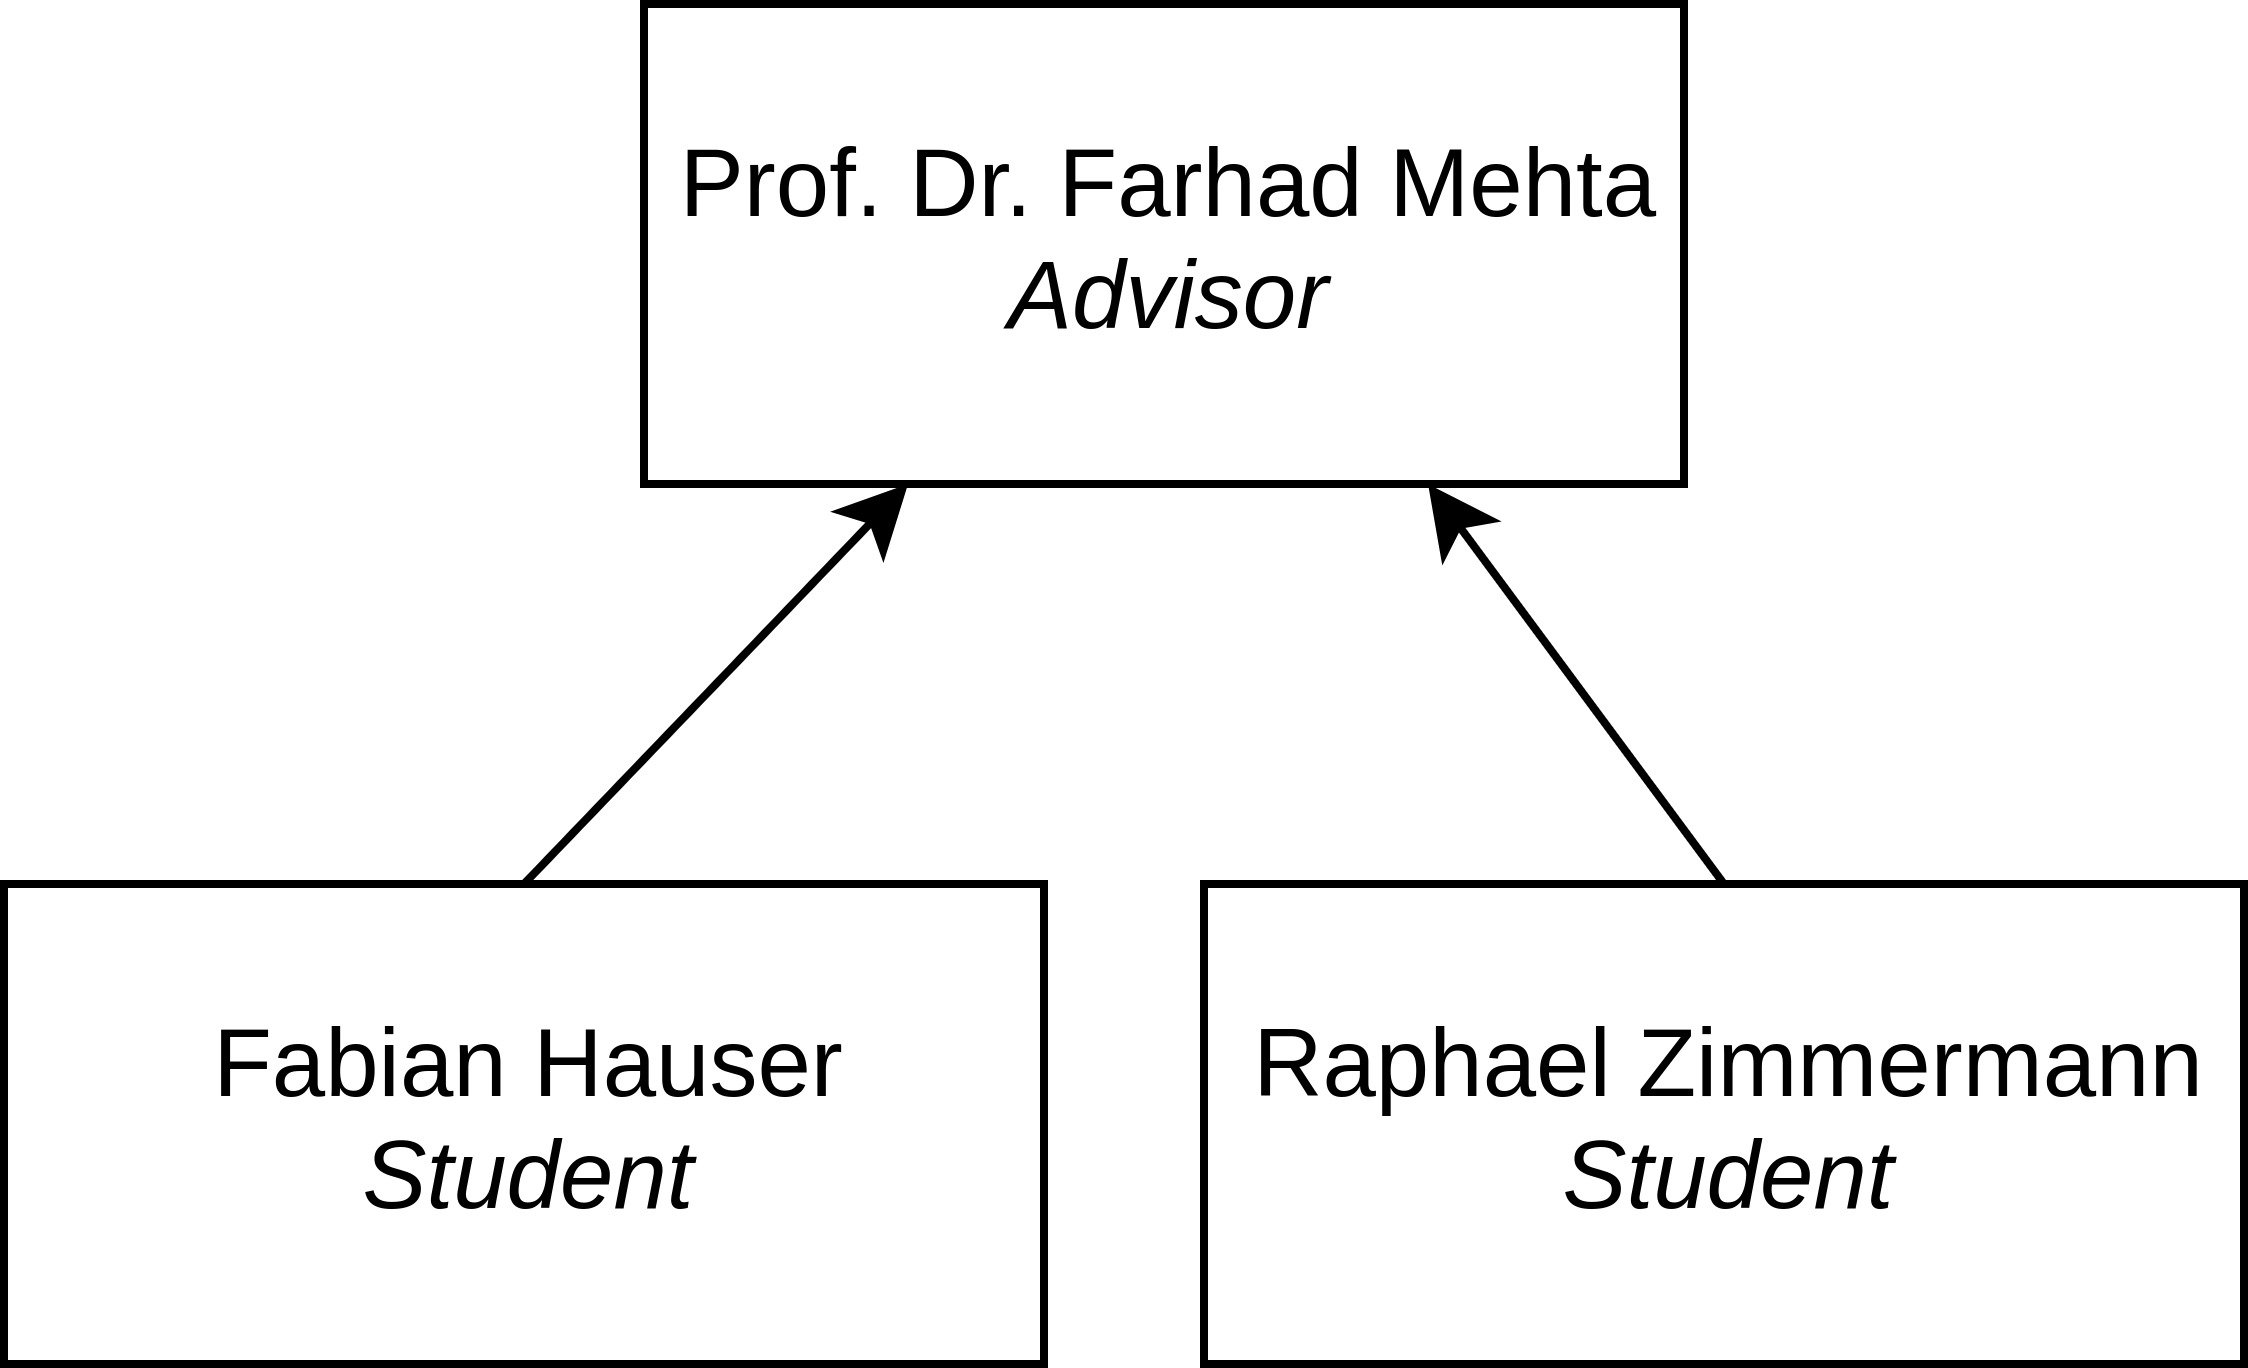
\includegraphics[width=0.5\linewidth]{resources/organigram}
	\caption[Organigram]{Project organization chart}
	\label{fig:organigram}
\end{figure}

\subsection{Roles}

Due to the small team size, most roles are performed by both team members.

\begin{description}
	\item[Raphael Zimmermann] project management, software engineering, quality assurance.
	\item[Fabian Hauser] infrastructure management, software engineering, quality assurance.
\end{description}

\section{Project Workflow}


\section{Risk Management}

\section{Infrastructure}

\section{Quality Measures}

\bibliographystyle{abbrv}
\bibliography{refs}

\end{document}
